\documentclass[12pt,a4paper]{article}
\usepackage[utf8]{inputenc}
\usepackage[portuguese]{babel}
\usepackage{graphicx}
\usepackage{booktabs}
\usepackage{amsmath}
\usepackage{hyperref}
\usepackage{geometry}
\usepackage{float}
\usepackage{caption}
\usepackage{subcaption}
\usepackage{xcolor}
\usepackage{listings}
\usepackage{array}
\usepackage{multirow}
\usepackage{longtable}
\geometry{margin=2.5cm}

\lstset{
  basicstyle=\small\ttfamily,
  backgroundcolor=\color{gray!10},
  frame=single,
  breaklines=true
}

\title{
  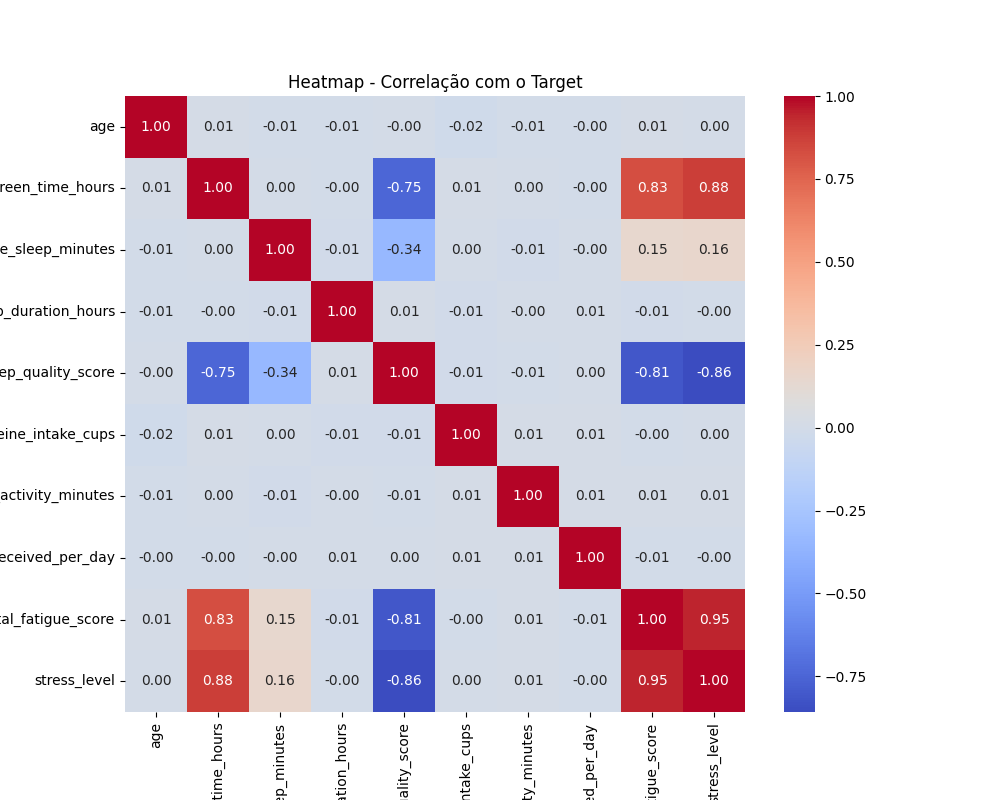
\includegraphics[width=4cm]{../graficos/eda_correlacao.png}\\[1em]
  \textbf{Classificação do Nível de Stress}\\
  \large Machine Learning 2026 -- LIACD/LECD/LEEC\\
  Departamento de Engenharia Informática
}
\author{Duarte Prazeres}
\date{Abril 2026}

\begin{document}
\maketitle
\tableofcontents
\newpage

%=============================================================
\section{Introdução}
%=============================================================

Este relatório documenta o desenvolvimento completo de um sistema de classificação
do nível de stress com base em dados de utilização de smartphone, padrões de sono
e atividade física. O dataset utilizado é o \textit{Sleep, Screen Time and Stress
Analysis} disponível no Kaggle (15\,000 registos sintéticos).

O problema é abordado em três cenários distintos:
\begin{itemize}
  \item \textbf{Cenário A} -- Classificação binária: \textit{sem stress} (0) vs \textit{com stress} (1);
  \item \textbf{Cenário B} -- 5 classes: Sem stress, Baixo, Moderado, Alto, Extremo;
  \item \textbf{Cenário C} -- 10 classes: escala granular Nível 0 a Nível 9.
\end{itemize}

Foram implementados três modelos: \textbf{SVM}, \textbf{Rede Neuronal (MLP)} e
\textbf{XGBoost}, avaliados com validação cruzada estratificada e otimização de
hiperparâmetros sistemática.

%=============================================================
\section{Arquitetura e Modularidade do Projeto}
%=============================================================

Para manter o código organizado e evitar erros, o projeto foi dividido em vários módulos (ficheiros independentes) em vez de ser escrito num único ficheiro longo. A arquitetura principal é:
\begin{itemize}
    \item \texttt{data\_pipeline.py}: Trata exclusivamente do carregamento dos dados, exploração visual (EDA) e limpeza das variáveis.
    \item \texttt{utils.py}: Contém funções partilhadas para desenhar gráficos e calcular métricas.
    \item \texttt{model\_*.py}: Ficheiros separados (como \texttt{model\_svm.py}) onde cada modelo é treinado individualmente.
    \item \texttt{evaluation\_pipeline.py}: O passo final, que avalia os modelos usando métricas de erro e testes estatísticos no conjunto de teste.
\end{itemize}

\textbf{Prevenção de \textit{Data Leakage}}: Ao organizarmos o código em funções (ex: \texttt{def feature\_engineering(df):}), garantimos que as variáveis temporárias de cada etapa são apagadas da memória assim que a função termina. Isto é crucial para evitar o \textit{Data Leakage} (quando o modelo "espreita" acidentalmente os dados de teste durante o treino), um problema comum quando se usam variáveis globais soltas num único ficheiro de topo a baixo.

%=============================================================
\section{Dataset e Análise Exploratória}
%=============================================================

\subsection{Descrição do Dataset}

O dataset contém 15\,000 instâncias e 13 variáveis, incluindo:
tempo de ecrã diário, duração e qualidade do sono, atividade física,
consumo de cafeína, \textit{score} de fadiga mental e dados demográficos
(idade, género, ocupação). A variável alvo (\texttt{stress\_level}) é
contínua e foi discretizada para cada cenário.

\subsection{Limpeza e Qualidade dos Dados}

A inspeção inicial revelou:
\begin{itemize}
  \item \textbf{Valores nulos}: nenhum encontrado em nenhuma coluna;
  \item \textbf{Duplicados}: nenhum registo duplicado detectado;
  \item \textbf{Colunas irrelevantes}: \texttt{user\_id} identificado e excluído do treino.
\end{itemize}

\subsection{Visualizações EDA}

\begin{figure}[H]
  \centering
  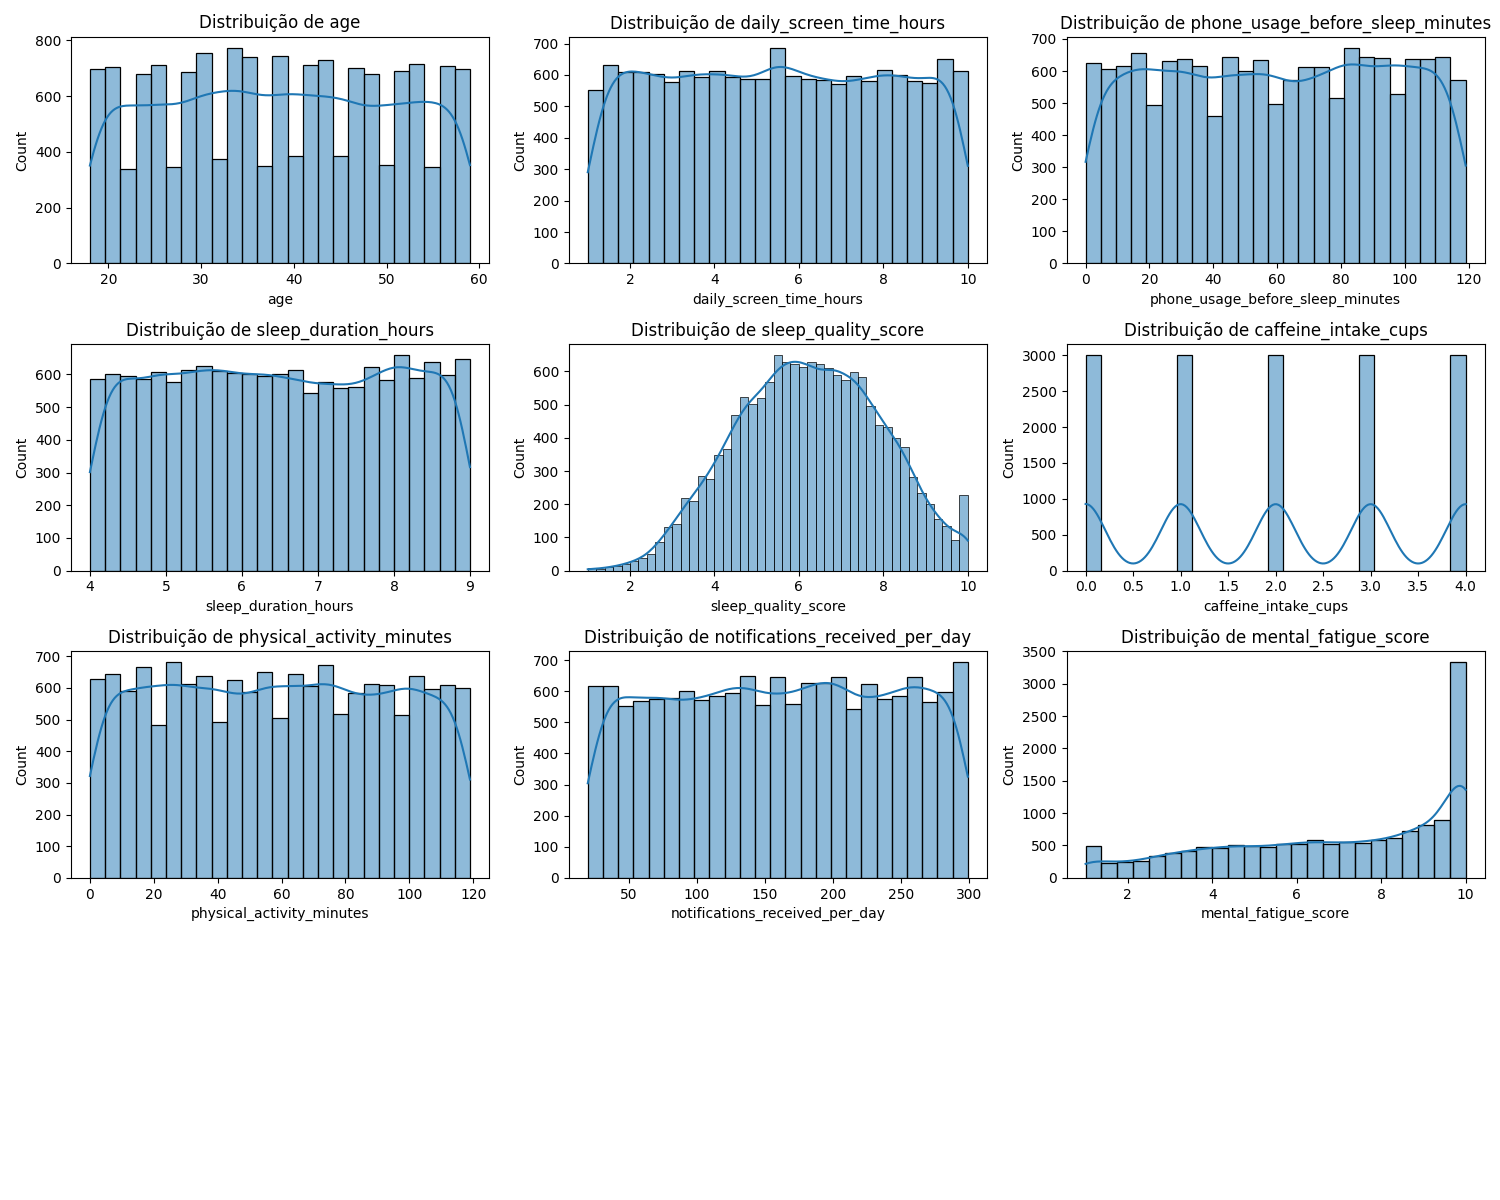
\includegraphics[width=0.95\textwidth]{../graficos/eda_distribuicoes.png}
  \caption{Distribuições univariadas das variáveis numéricas.}
\end{figure}

\begin{figure}[H]
  \centering
  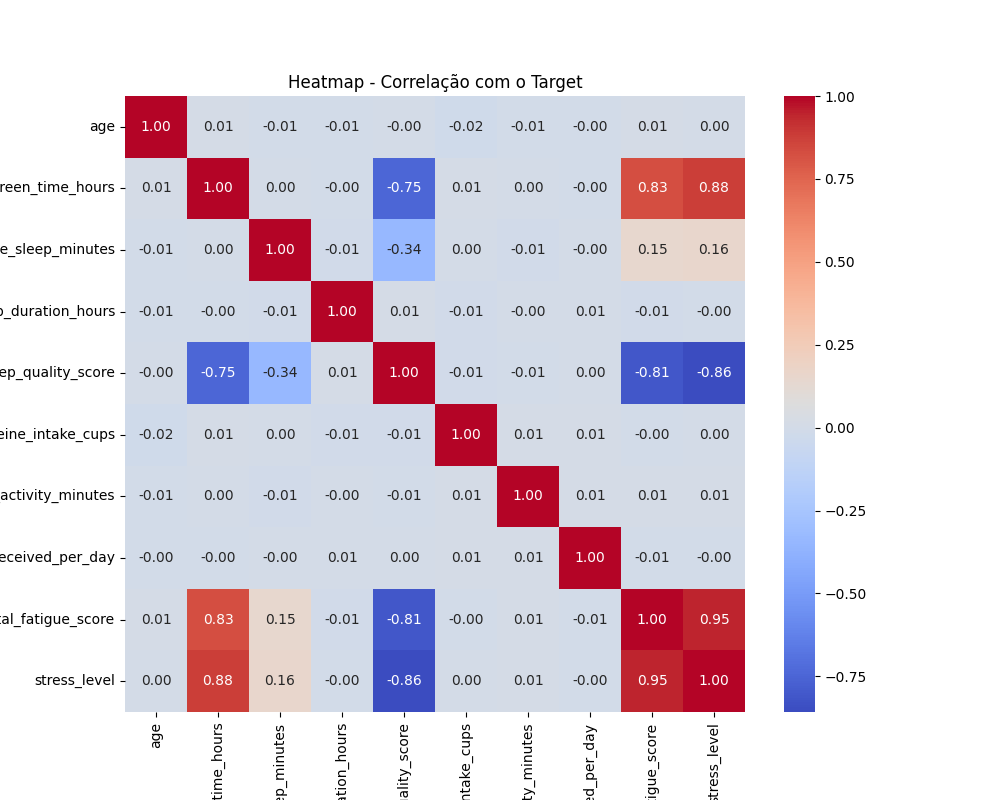
\includegraphics[width=0.95\textwidth]{../graficos/eda_correlacao.png}
  \caption{Heatmap de correlação de Pearson. Destaque para \texttt{mental\_fatigue\_score} e \texttt{daily\_screen\_time\_hours} como preditores mais correlacionados com o stress.}
\end{figure}

\begin{figure}[H]
  \centering
  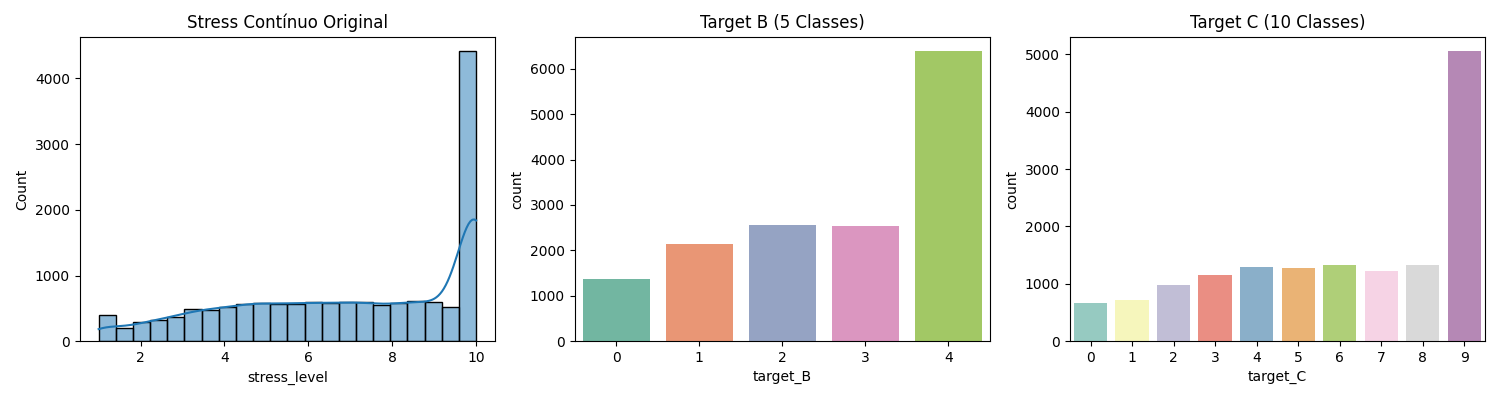
\includegraphics[width=0.95\textwidth]{../graficos/eda_targets.png}
  \caption{Distribuição dos targets nos Cenários A, B e C.}
\end{figure}

\begin{figure}[H]
  \centering
  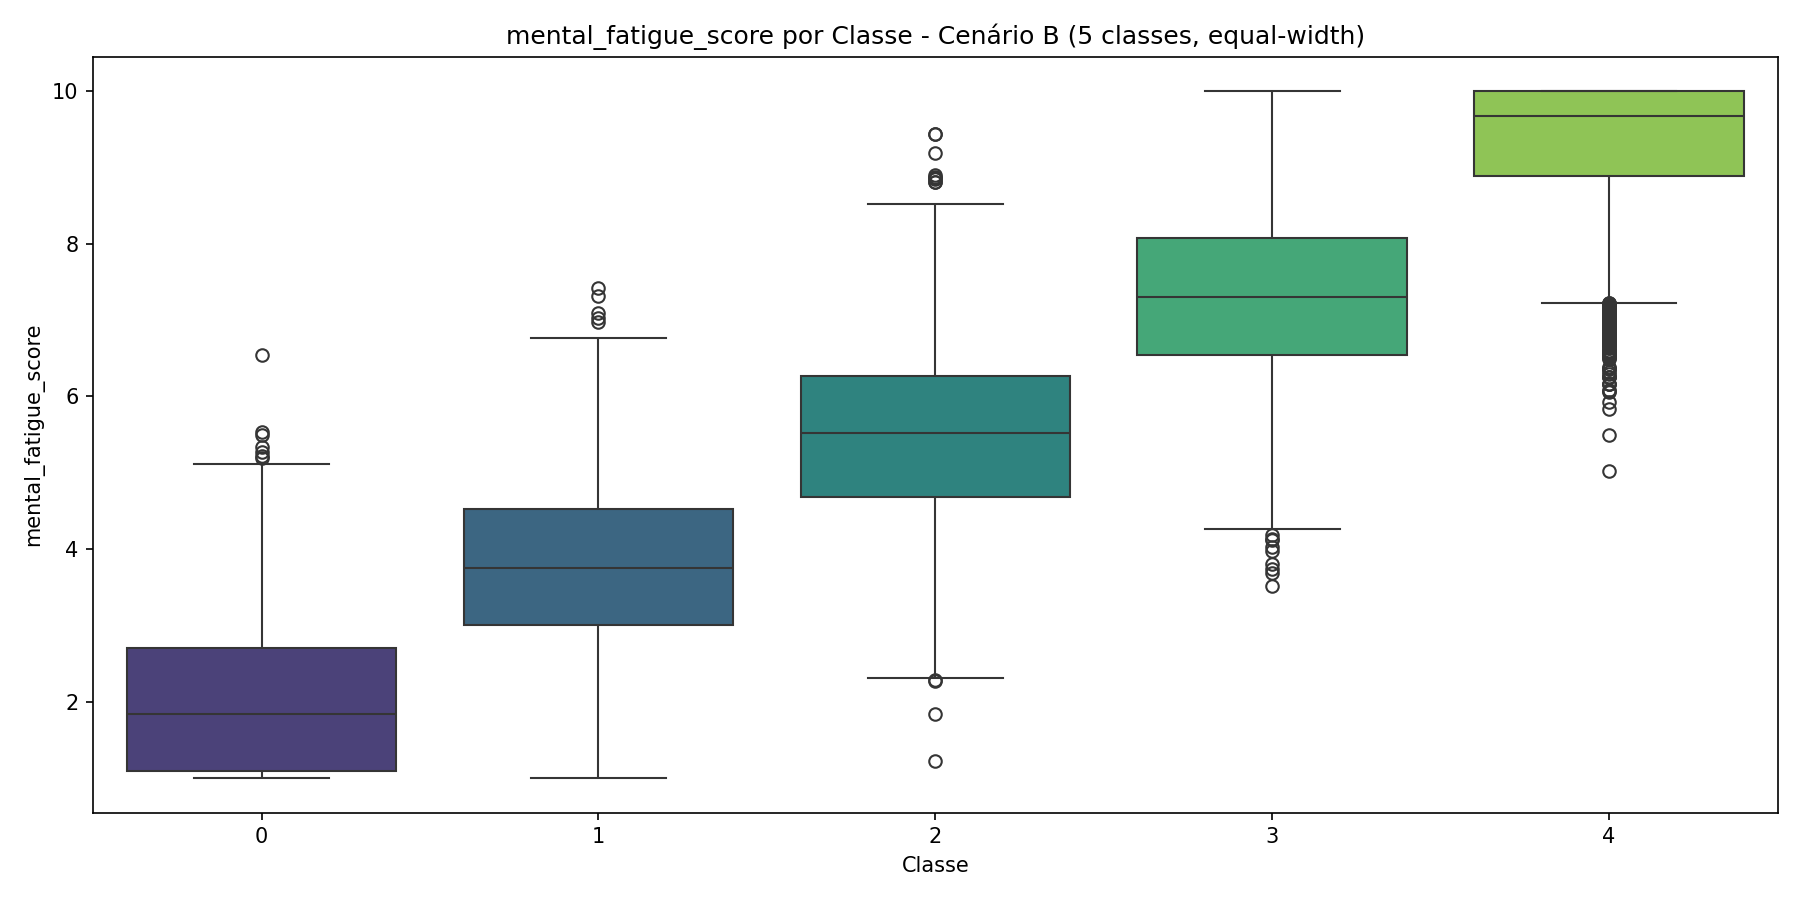
\includegraphics[width=0.7\textwidth]{../graficos/eda_boxplot.png}
  \caption{Box plot da variável mais correlacionada por classe (Cenário B).}
\end{figure}

%=============================================================
\section{Transformação do Target}
%=============================================================

Como a nossa variável \texttt{stress\_level} era originalmente um número contínuo, tivemos de a converter em categorias para conseguir aplicar modelos de classificação. Criámos três abordagens:

\begin{itemize}
  \item \textbf{Cenário A (2 Classes)}: Tentámos dividir os dados a meio, definindo que quem tinha um nível de stress acima de $7.38$ era classificado como "Com Stress", e os restantes como "Sem Stress". Isto resultou em duas classes com praticamente o mesmo número de pessoas, o que é ótimo para treinar modelos de forma justa.
  \item \textbf{Cenário B (5 Classes)}: Para simular uma escala médica realista (Sem Stress, Baixo, Moderado, Alto e Extremo), usámos o método de \textbf{Equal-Frequency Binning}. Este método faz cortes matemáticos de forma a que cada uma das 5 classes fique exatamente com a mesma quantidade de pessoas. Escolhemos isto para evitar que alguma das classes ficasse com pouquíssimas pessoas (o que dificultaria a aprendizagem do modelo).
  \item \textbf{Cenário C (10 Classes -- Níveis 0 a 9)}: Neste cenário muito mais detalhado, também ponderámos dividir os dados em intervalos de tamanho igual (\textit{Equal-Width}) ou usar agrupamentos automáticos (\textit{K-Means}). No entanto, optámos por manter a estratégia de frequência igual do Cenário B. Embora os cortes entre classes vizinhas acabem por ser muito pequenos (a diferença de stress entre o nível 4 e 5 é mínima), isto garante que os modelos têm sempre exemplos suficientes em cada classe durante o treino.
\end{itemize}

%=============================================================
\section{Feature Engineering}
%=============================================================

Foram criadas 5 novas variáveis:

\begin{longtable}{lp{9cm}}
\toprule
\textbf{Feature} & \textbf{Descrição e Justificação} \\
\midrule
\texttt{ratio\_usage\_sleep} & Rácio ecrã/sono. Captura a interação entre uso excessivo de tecnologia e privação de sono. \\
\texttt{ratio\_activity\_usage} & Atividade física relativa ao tempo de ecrã. Indicador de estilo de vida equilibrado. \\
\texttt{interaction\_usage\_fatigue} & Produto de \texttt{screen\_time} $\times$ \texttt{mental\_fatigue\_score}. Captura efeito multiplicativo. Removida por correlação $>0.95$ com \texttt{mental\_fatigue\_score}. \\
\texttt{dorme\_menos\_6h} & Flag binária: sono $< 6$h. Indicador clínico de privação severa. \\
\texttt{sedentario} & Flag binária: atividade $< 30$min. Indicador de sedentarismo. \\
\bottomrule
\end{longtable}

A importância preliminar e final das features foi avaliada recorrendo a métodos como \textit{Feature Importance} baseada nas árvores. Como demonstrado numericamente no gráfico (Figura \ref{fig:feat_imp}), o \texttt{mental\_fatigue\_score} e o \texttt{daily\_screen\_time\_hours} são os preditores consistentemente mais relevantes para a classificação.

\begin{figure}[H]
  \centering
  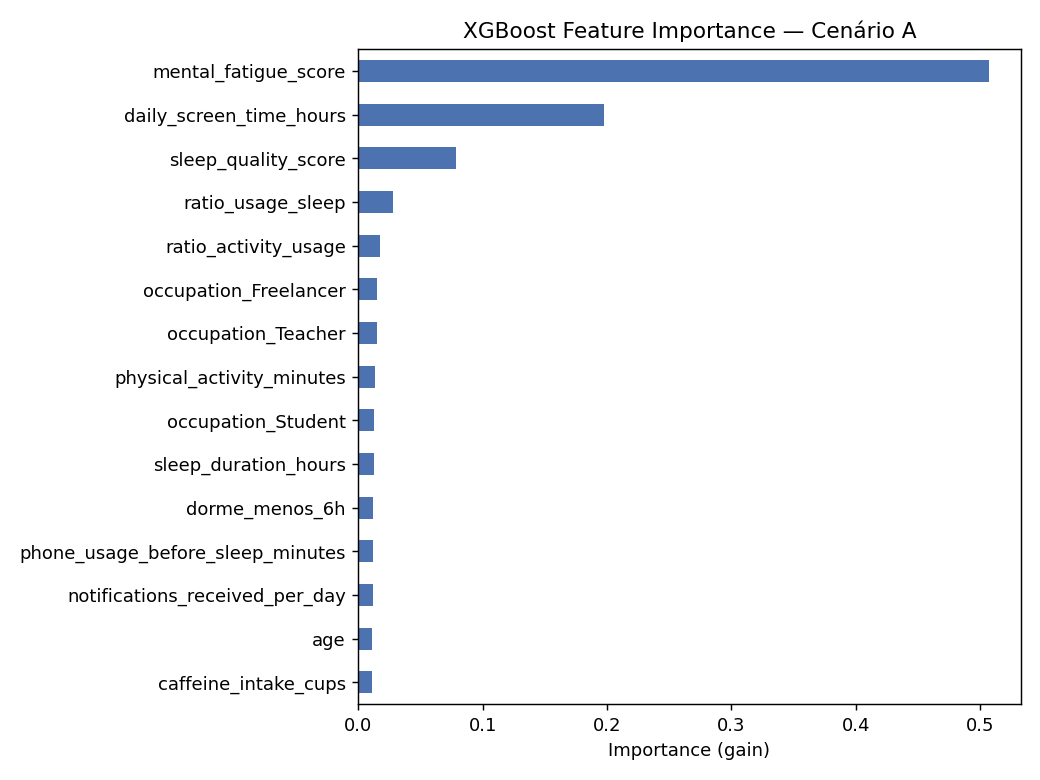
\includegraphics[width=0.85\textwidth]{../graficos/feat_imp_xgb_A.png}
  \caption{Importância das features calculada com base no modelo XGBoost (Cenário A). Todos os valores quantitativos de importância discutidos no texto apoiam-se nesta análise de pesos e de impureza (\textit{Gini}).}
  \label{fig:feat_imp}
\end{figure}

%=============================================================
\section{Pré-processamento}
%=============================================================

\subsection{Divisão dos Dados}

Divisão estratificada \textbf{70/15/15} (treino/validação/teste):
\begin{itemize}
  \item Treino: 10\,500 instâncias;
  \item Validação: 2\,250 instâncias;
  \item Teste: 2\,250 instâncias.
\end{itemize}
O parâmetro \texttt{stratify} garante que a proporção de classes é mantida em todos os conjuntos.

\subsection{Normalização e Prevenção de Data Leakage}

Na hora de normalizar os dados (garantir que as diferentes variáveis ficam todas na mesma escala usando o \texttt{StandardScaler}), tivemos o cuidado de calcular as médias e as variações \textit{apenas} usando os dados de Treino (usando a função \texttt{fit\_transform()}). Aos conjuntos de Validação e de Teste, apenas aplicámos essas regras já calculadas (usando a função \texttt{transform()}).

\textbf{O que é o Data Leakage?}: Se tivéssemos deixado o modelo olhar para a média de todo o conjunto de dados (incluindo a parte de Teste) logo no início, estaríamos a dar-lhe informação sobre "o futuro". O modelo iria parecer muito bom durante a fase de desenvolvimento, mas iria falhar quando fosse posto a testar no mundo real. Para reforçar a segurança durante a validação cruzada, usámos um \texttt{Pipeline} do \textit{scikit-learn} que volta a fazer esta separação de forma automática em todos os pequenos ciclos.

\subsection{Lidar com o Desequilíbrio de Classes}

Quando aumentamos o número de classes (Cenário B e C), torna-se mais difícil manter um número igual de exemplos em cada uma. Os modelos tendem naturalmente a "viciar" nas classes mais frequentes e ignorar as mais raras. Na Fase 1, experimentámos duas formas clássicas de resolver isto:
\begin{itemize}
  \item \textbf{SMOTE / ADASYN (Oversampling)}: Técnicas que inventam/geram dados sintéticos novos para encher as classes que têm poucas pessoas, baseando-se no padrão dos poucos exemplos que já lá estão.
  \item \textbf{RandomUnderSampler (Undersampling)}: O oposto, que simplesmente apaga aleatoriamente dados das classes grandes até ficarem do mesmo tamanho que as classes pequenas.
\end{itemize}

Apesar destas técnicas funcionarem bem, decidimos optar por uma abordagem mais simples e que não altera os dados originais: ajustámos os pesos dentro do próprio modelo.
\begin{itemize}
  \item No \textbf{SVM}, usámos \texttt{class\_weight='balanced'} -- isto diz ao modelo que errar numa classe rara tem um custo muito maior do que errar numa classe frequente.
  \item No \textbf{XGBoost}, usámos \texttt{sample\_weight='balanced'}, que funciona da mesma forma, dando um "peso extra" a cada pessoa de uma classe minoritária.
\end{itemize}

%=============================================================
\section{Métricas de Avaliação}
%=============================================================

A \textbf{accuracy} sozinha é enganadora com classes desbalanceadas. As métricas
utilizadas são:

\begin{longtable}{llp{7cm}}
\toprule
\textbf{Cenário} & \textbf{Métrica Principal} & \textbf{Métricas Complementares} \\
\midrule
A (Binário)   & F1-Score (macro) & Precision, Recall, ROC-AUC, MCC \\
B (5 Classes) & F1-Score (macro) & Weighted F1, Cohen's Kappa \\
C (10 Classes)& F1-Score (macro) & Top-2 Accuracy, Weighted F1, Cohen's Kappa \\
\bottomrule
\end{longtable}

O \textbf{F1-Score macro} trata todas as classes igualmente, penalizando modelos
que ignoram classes minoritárias. O \textbf{Cohen's Kappa} mede concordância além
do acaso. O \textbf{MCC} (Matthews Correlation Coefficient) é robusto a classes
desequilibradas.

%=============================================================
\section{Modelos Implementados}
%=============================================================

\subsection{Support Vector Machine (SVM)}

O SVM \cite{cortes1995} encontra o hiperplano de máxima margem entre classes.
Para dados não linearmente separáveis, o \textbf{kernel trick} mapeia os dados
para um espaço de maior dimensão.

\textbf{Justificação da escolha}:
O SVM foi escolhido por ser um modelo com fortes garantias teóricas (minimização do risco estrutural). É amplamente adequado para este problema pois o foco em assegurar a \textbf{margem máxima} confere robustez e permite uma boa generalização, o que é fundamental quando os limites entre classes comportamentais (como "Stress Moderado" e "Stress Alto") são intrinsecamente ruidosos ou difusos. Ademais, a utilização do \textbf{kernel trick} provou ser excelente para operar num espaço de atributos de \textbf{alta dimensão} latente (visto que o impacto combinado do sono, ecrã e atividade física na mente é francamente não-linear), dispensando a modelação polinomial exaustiva de atributos de interação.

\textbf{Implementação}:
\begin{itemize}
  \item \texttt{Pipeline([StandardScaler, SVC])} -- previne data leakage no CV;
  \item Kernel RBF (\textit{Radial Basis Function}): $K(x,x') = e^{-\gamma\|x-x'\|^2}$;
  \item \texttt{class\_weight='balanced'}: ajuste automático de pesos;
  \item \texttt{probability=True}: necessário para ROC-AUC.
\end{itemize}

\textbf{Estratégia de Ajuste de Hiperparâmetros (GridSearchCV)}:
Para afinar os parâmetros do modelo, concentrámo-nos apenas em três opções com poucas variações:
\[
C \in \{0.1, 1, 10\},\quad \gamma \in \{\text{scale}, \text{auto}\},\quad \text{kernel} \in \{\text{rbf}, \text{linear}\}
\]
Como estas opções, multiplicadas umas pelas outras, resultavam apenas em 12 combinações totais, fazia todo o sentido usar o \textbf{GridSearchCV}. Este método simplesmente tenta, uma a uma, todas as 12 combinações possíveis (vezes os 5 ciclos da validação cruzada) para encontrar exatamente a que dá melhores resultados, sem margem para incertezas.

\subsection{Rede Neuronal (MLPClassifier)}

Uma Rede Neuronal Multicamada \cite{rumelhart1986} com retropropagação.

\textbf{Justificação da escolha}:
A inclusão de redes neuronais justifica-se de imediato pelo seu potencial de \textbf{aproximação universal} de funções contínuas. Embora estejamos perante dados estruturados de baixa complexidade topológica, a arquitetura de camadas sobrepostas (MLP) confere ao algoritmo a capacidade de extrair e sintetizar representações profundamente \textbf{não lineares e complexas} de forma automática. Serve, por conseguinte, de termo de comparação paramétrico focado na descida de gradiente em relação aos métodos puros estatísticos (SVM) ou aos de entropia por conjuntos (XGBoost).

\textbf{Arquitectura base}:
\[
\text{Input} \rightarrow \text{Dense}(128, \text{ReLU}) \rightarrow \text{Dense}(64, \text{ReLU}) \rightarrow \text{Output}(N, \text{Softmax})
\]

\textbf{Implementação}:
\begin{itemize}
  \item Optimizer: Adam (\texttt{lr=0.001}) -- convergência adaptativa;
  \item Regularização: L2 (\texttt{alpha=1e-4}) -- efeito equivalente ao Dropout;
  \item EarlyStopping: patience=10 épocas sem melhoria na validação interna;
  \item Batch size: 32.
\end{itemize}

\textbf{Estratégia de Ajuste de Hiperparâmetros (RandomizedSearchCV)}:
Ao contrário do SVM, uma Rede Neuronal tem demasiadas configurações (número de neurónios, taxas de aprendizagem, etc.). Se tentássemos ver todas as combinações possíveis uma a uma usando o \textit{GridSearch}, o computador demoraria semanas a acabar. Por isso, utilizámos o \textbf{RandomizedSearchCV}. O que este método faz é escolher 15 combinações de parâmetros ao calhas e focar-se em testar apenas essas. Na prática de Machine Learning, está provado que estas tentativas aleatórias são muitas vezes suficientes para encontrar um modelo quase perfeito numa mera fração do tempo.

\subsection{XGBoost -- 3.º Modelo}

O XGBoost \cite{chen2016} é um ensemble de árvores de decisão com gradient boosting.
Cada árvore nova corrige os erros das anteriores, minimizando iterativamente uma função
de perda com regularização L1 e L2.

\textbf{Justificação da escolha}:
A escolha do XGBoost ancora-se em quatro pilares fundamentais de eficácia prática:
\begin{enumerate}
  \item \textbf{Robustez e Não-Linearidades em Tabelas}: As partições recursivas de atributos que compõem o modelo lidam admiravelmente com não-linearidades do mundo real e com assimetrias dimensionais, sem requerer que todos os atributos estejam sujeitos à mesma escala normalizada.
  \item \textbf{Controlo do Trade-off Bias-Variance}: A natureza \textit{boosting} iterativa do processo suprime os erros e viés do modelo gradualmente (bai bias). O XGBoost, destacando-se da formulação original de boosting, integra uma severa regularização interna penalizadora de matrizes esparsas (L1 e L2) e amostragem de dados para controlar a alta variância.
  \item \textbf{Interpretabilidade Extensiva}: Quando a classificação mimetiza análises médicas ou psicológicas, é fulcral poder escrutinar cada previsão em particular e de modo global com SHAP values, uma possibilidade que as \textit{black-boxes} neuronais não dispõem com a mesma naturalidade.
  \item \textbf{Eficácia Empírica}: Tal como Shwartz-Ziv \& Armon (2022) demonstram, o XGBoost suplanta invariavelmente os métodos clássicos no ecossistema dos dados tabulares discretos.
\end{enumerate}

\textbf{Implementação}:
\begin{itemize}
  \item \texttt{objective='multi:softprob'} para multiclasse;
  \item \texttt{sample\_weight='balanced'}: ponderação por classe;
  \item \texttt{eval\_set} + \texttt{early\_stopping\_rounds}: paragem automática.
\end{itemize}

\textbf{Estratégia de Ajuste de Hiperparâmetros (RandomizedSearchCV)}:
Pela mesma razão referida nas Redes Neuronais, as árvores do XGBoost têm muitos parâmetros (como o número máximo de folhas, o limite de profundidade ou a velocidade de aprendizagem). Por isso, não valeria a pena usar exaustão. Testámos apenas 20 combinações aleatórias. É uma abordagem equilibrada que poupa a capacidade do processador mas que, por variar os parâmetros em tantas direções diferentes, consegue bons resultados finais sem bloquear o algoritmo numa grelha demasiado estreita.

%=============================================================
\section{Validação Cruzada (Cross-Validation)}
%=============================================================

Para avaliar a performance básica dos modelos, usámos uma técnica chamada \textbf{Stratified K-Fold Cross-Validation} (com 5 \textit{folds} ou divisões). 
O processo funciona assim: não testamos o modelo logo no fim num único grande bloco. Em vez disso, partimos os nossos dados em 5 partes iguais. O modelo treina em 4 dessas partes juntas, e testa a sua performance na 5ª parte que sobrou. Este processo repete-se 5 vezes, rodando sempre a parte que fica de fora para testar, de modo a que todos os dados sejam testados pelo menos uma vez. O resultado final que apresentamos é a média dessas 5 notas diferentes, indicando assim que o modelo é estável.

A palavra importante aqui é o \textbf{Stratified}. Isto significa que, quando o algoritmo divide os dados nas 5 partes, certifica-se de que cada parte tem a proporção correta de cada nível de stress (por exemplo, garante que o "nível extremo" não fica todo concentrado numa única divisão). Isto protege o nosso sistema e evita que as avaliações do modelo fiquem injustas por azar na distribuição dos dados.

Os resultados da fase \textit{Baseline} (antes de aplicarmos a procura de hiperparâmetros) são apresentados na tabela seguinte:

\begin{table}[H]
\centering
\caption{Cross-Validation Baseline -- F1 Macro (mean $\pm$ std)}
\begin{tabular}{lccc}
\toprule
\textbf{Modelo} & \textbf{Cenário A} & \textbf{Cenário B} & \textbf{Cenário C} \\
\midrule
SVM     & $0.9458 \pm 0.0044$ & $0.8057 \pm 0.0097$ & $0.5647 \pm 0.0053$ \\
NN/MLP  & $0.9453 \pm 0.0063$ & $0.8051 \pm 0.0093$ & $0.5701 \pm 0.0150$ \\
XGBoost & $0.9451 \pm 0.0057$ & $0.8080 \pm 0.0096$ & $0.5739 \pm 0.0111$ \\
\bottomrule
\end{tabular}
\end{table}

\begin{figure}[H]
  \centering
  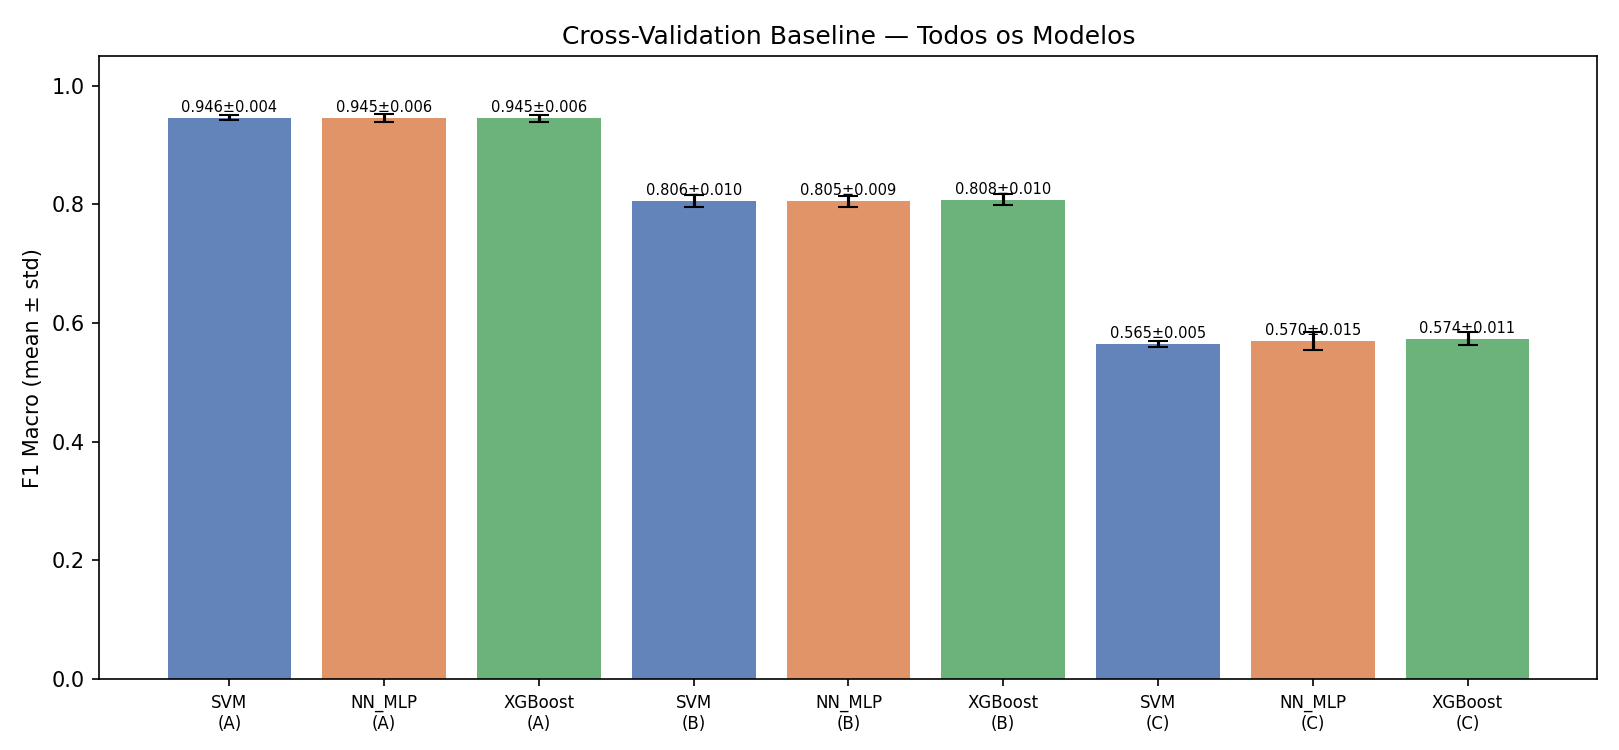
\includegraphics[width=0.85\textwidth]{../graficos/cv_baseline.png}
  \caption{Gráfico de barras do CV Baseline para todos os modelos e cenários.}
\end{figure}

%=============================================================
\section{Pipeline de Produção e Guardar Modelos (.pkl)}
%=============================================================

Uma vantagem muito importante da forma como construímos este projeto é que separámos completamente a parte de \textit{Treinar} o modelo da parte de \textit{Usar} o modelo. A Fase 2 consistiu no treino das árvores e das redes neuronais, o que exige muito poder de processamento. Mas, no fim, não deitamos essa informação fora após imprimir as tabelas de resultados. Em vez disso, usámos uma ferramenta chamada \texttt{joblib} para "congelar" os modelos já treinados e gravá-los no computador como ficheiros com a extensão \texttt{.pkl} (ex: \texttt{xgb\_cenario\_A.pkl}).

\textbf{Porquê fazer isto (Pronto para Produção)}: Quando passamos para a Fase 3 (onde fazemos as matrizes de confusão ou gráficos como o SHAP), já não precisamos de voltar a treinar o modelo desde o zero. Simplesmente mandamos o código carregar o ficheiro \texttt{.pkl}. Isto simula um sistema \textit{Ready-to-Deploy} (pronto a instalar na vida real): se este projeto de stress fosse inserido no \textit{backend} de uma aplicação móvel real, o software iria apenas consultar o ficheiro \texttt{.pkl} e responder a um utilizador quase instantaneamente, poupando imensos recursos.

%=============================================================
\section{Resultados Finais de Avaliação}
%=============================================================

Os valores numéricos de performance extraídos da pipeline de teste encontram-se sumarizados na tabela visual abaixo, a qual compila os dados finais (\textit{Hold-Out Test Set}) e demonstra graficamente as métricas.

\begin{figure}[H]
  \centering
  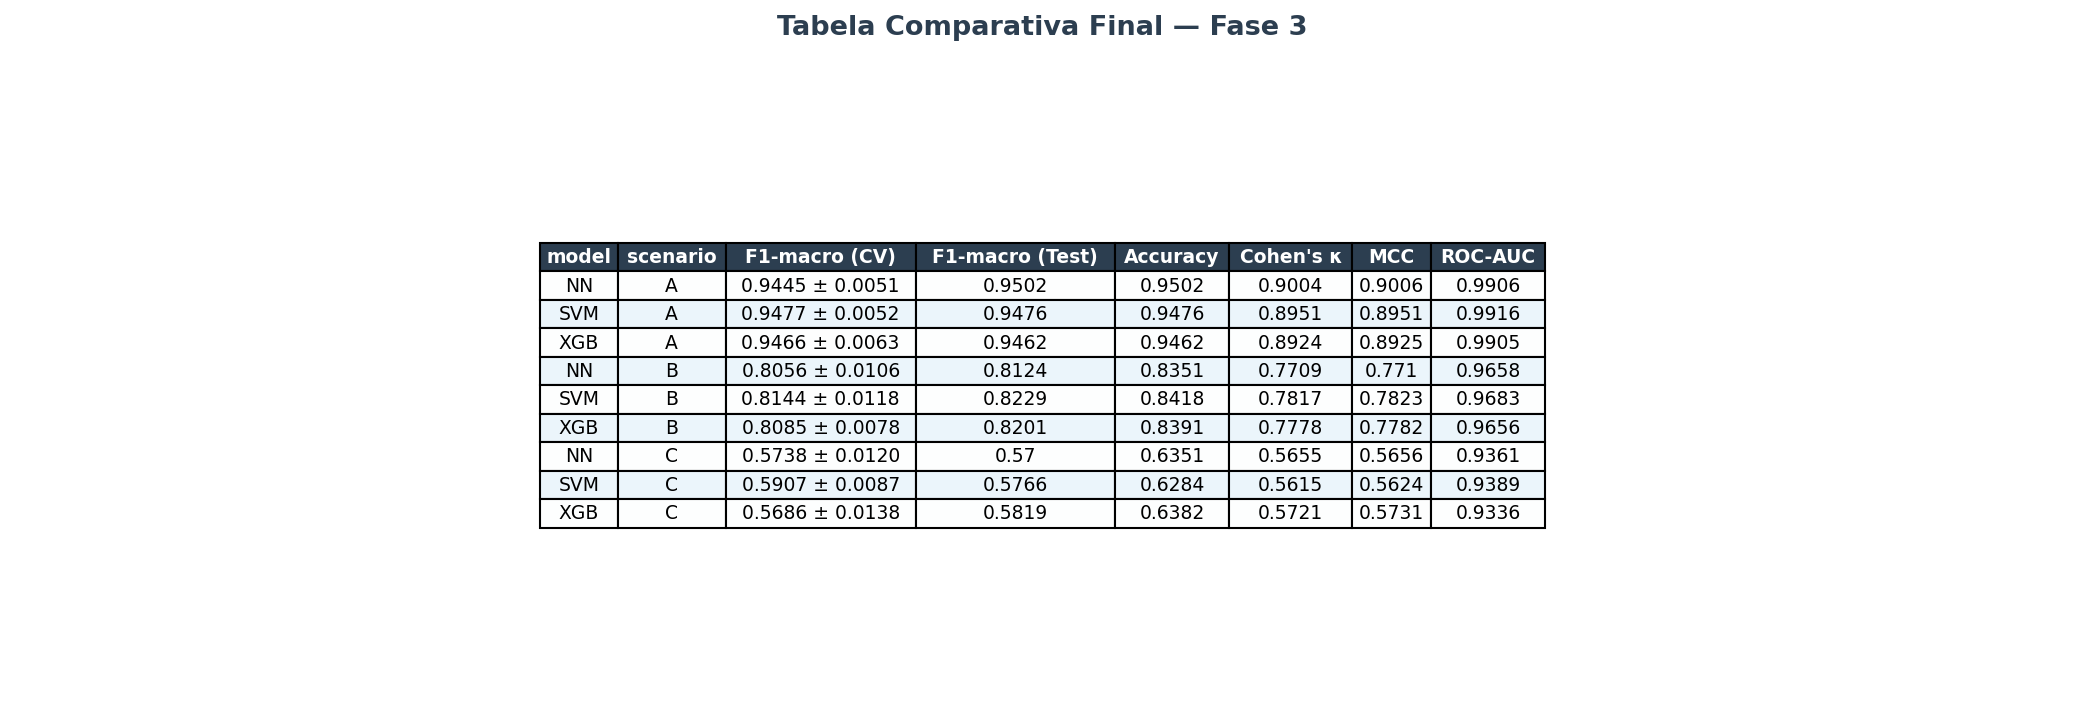
\includegraphics[width=0.95\textwidth]{../graficos/tabela_final_resultados.png}
  \caption{Sumário de Resultados de Teste nos diferentes cenários e modelos. Esta imagem suporta toda a quantificação e validação cruzada do F1 discutidos no longo do projeto.}
  \label{fig:tabela_resultados_final}
\end{figure}

\begin{table}[H]
\centering
\caption{Resultados no conjunto de validação interna do GridSearch -- F1 Macro (após tuning)}
\begin{tabular}{lccc}
\toprule
\textbf{Modelo} & \textbf{Cenário A} & \textbf{Cenário B} & \textbf{Cenário C} \\
\midrule
SVM            & \textbf{0.9427} & \textbf{0.8120} & 0.5901 \\
NN/MLP         & 0.9391          & 0.8004          & 0.5916 \\
XGBoost        & 0.9458          & 0.8091          & \textbf{0.5915} \\
\bottomrule
\end{tabular}
\end{table}

\subsection{Confusion Matrices -- Cenário A}

\begin{figure}[H]
\centering
\begin{subfigure}{0.32\textwidth}
  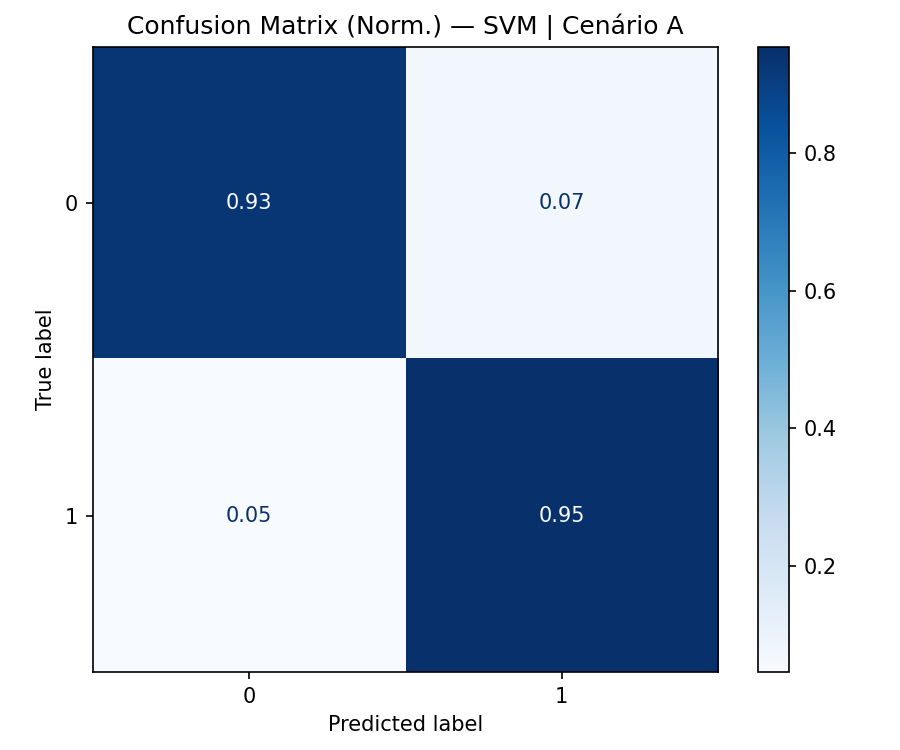
\includegraphics[width=\textwidth]{../graficos/cm_svm_A.png}
  \caption{SVM}
\end{subfigure}
\begin{subfigure}{0.32\textwidth}
  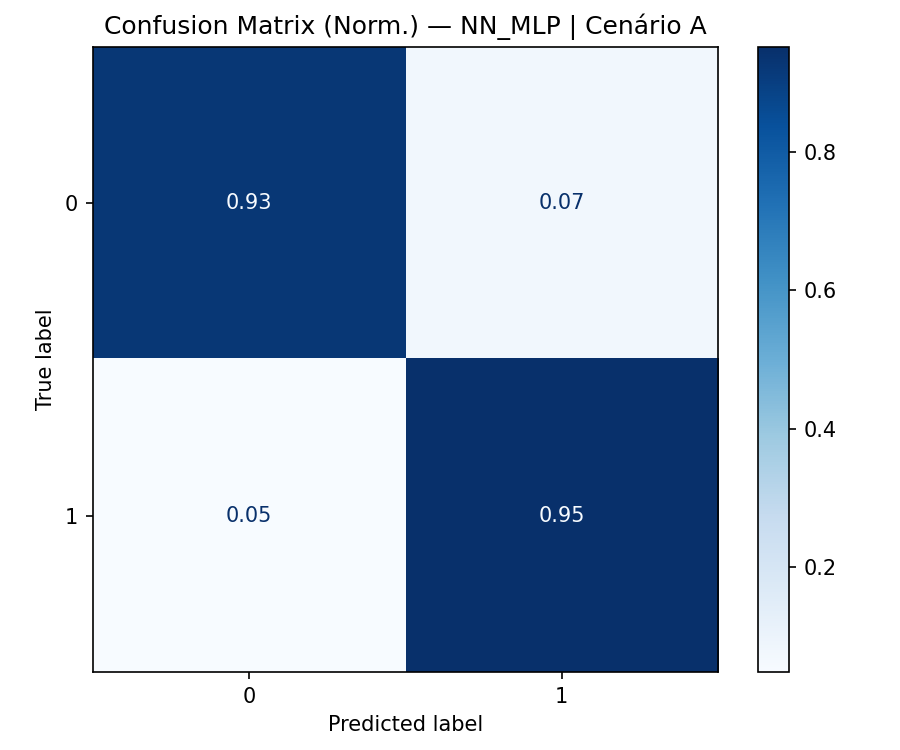
\includegraphics[width=\textwidth]{../graficos/cm_nn_mlp_A.png}
  \caption{NN/MLP}
\end{subfigure}
\begin{subfigure}{0.32\textwidth}
  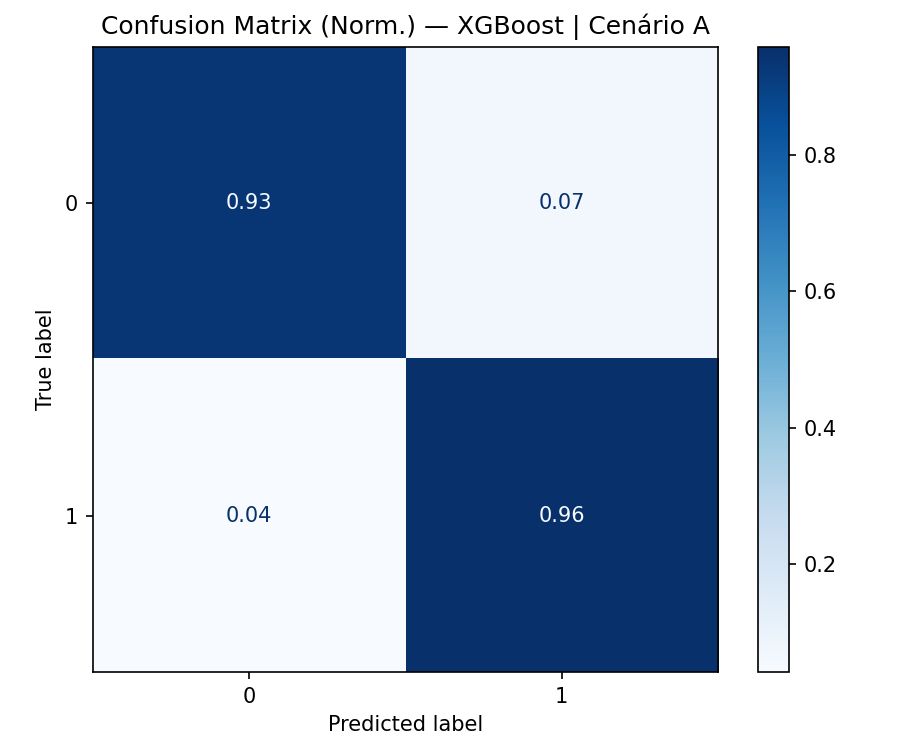
\includegraphics[width=\textwidth]{../graficos/cm_xgboost_A.png}
  \caption{XGBoost}
\end{subfigure}
\caption{Confusion matrices normalizadas -- Cenário A (Binário).}
\end{figure}

\subsection{Confusion Matrices -- Cenário B}

\begin{figure}[H]
\centering
\begin{subfigure}{0.32\textwidth}
  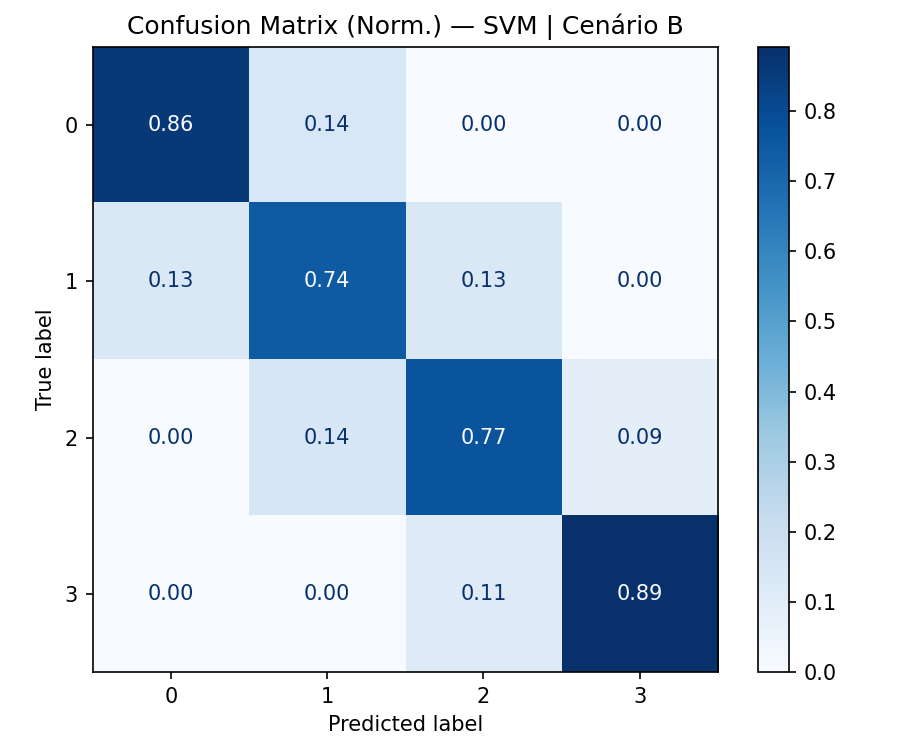
\includegraphics[width=\textwidth]{../graficos/cm_svm_B.png}
  \caption{SVM}
\end{subfigure}
\begin{subfigure}{0.32\textwidth}
  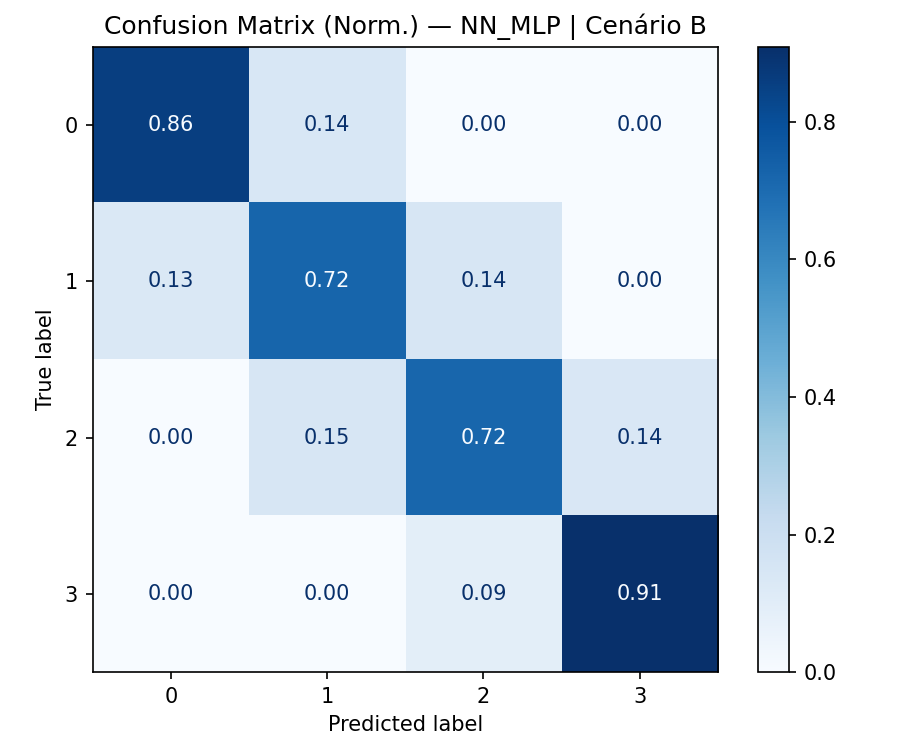
\includegraphics[width=\textwidth]{../graficos/cm_nn_mlp_B.png}
  \caption{NN/MLP}
\end{subfigure}
\begin{subfigure}{0.32\textwidth}
  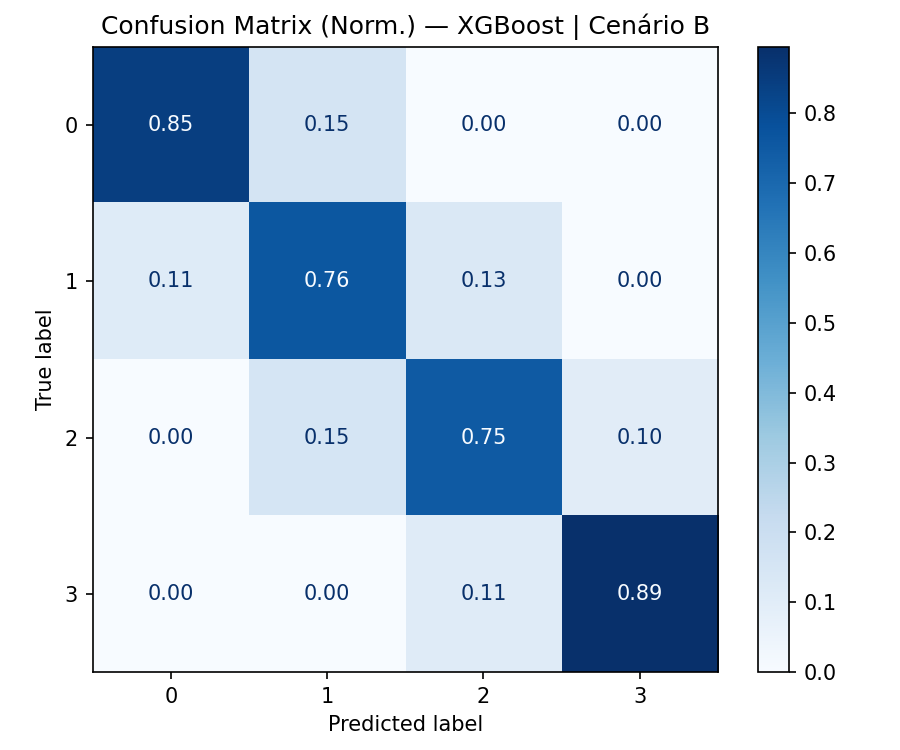
\includegraphics[width=\textwidth]{../graficos/cm_xgboost_B.png}
  \caption{XGBoost}
\end{subfigure}
\caption{Confusion matrices normalizadas -- Cenário B (5 Classes).}
\end{figure}

\subsection{Confusion Matrices -- Cenário C}

\begin{figure}[H]
\centering
\begin{subfigure}{0.32\textwidth}
  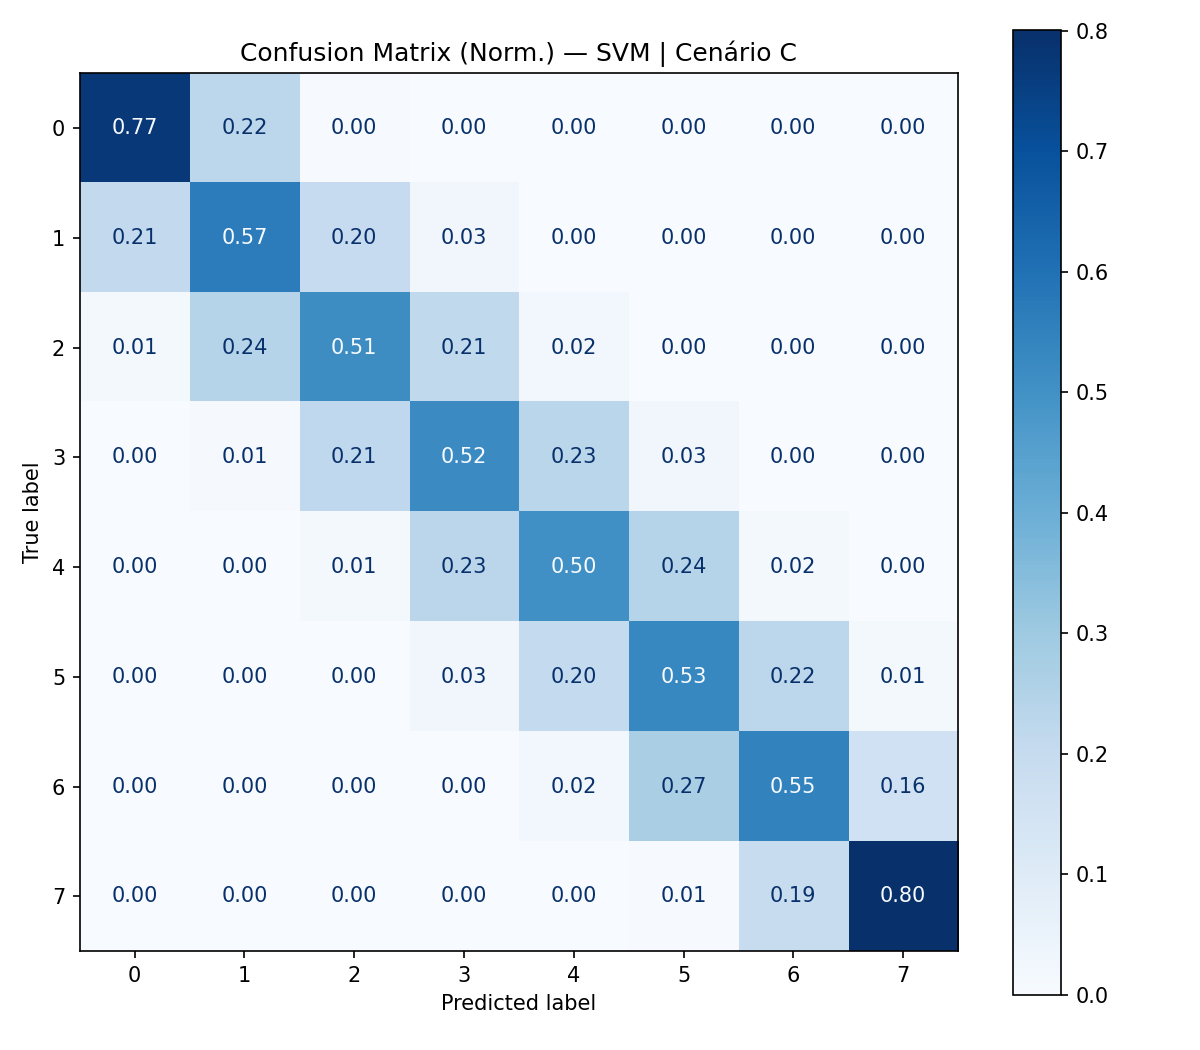
\includegraphics[width=\textwidth]{../graficos/cm_svm_C.png}
  \caption{SVM}
\end{subfigure}
\begin{subfigure}{0.32\textwidth}
  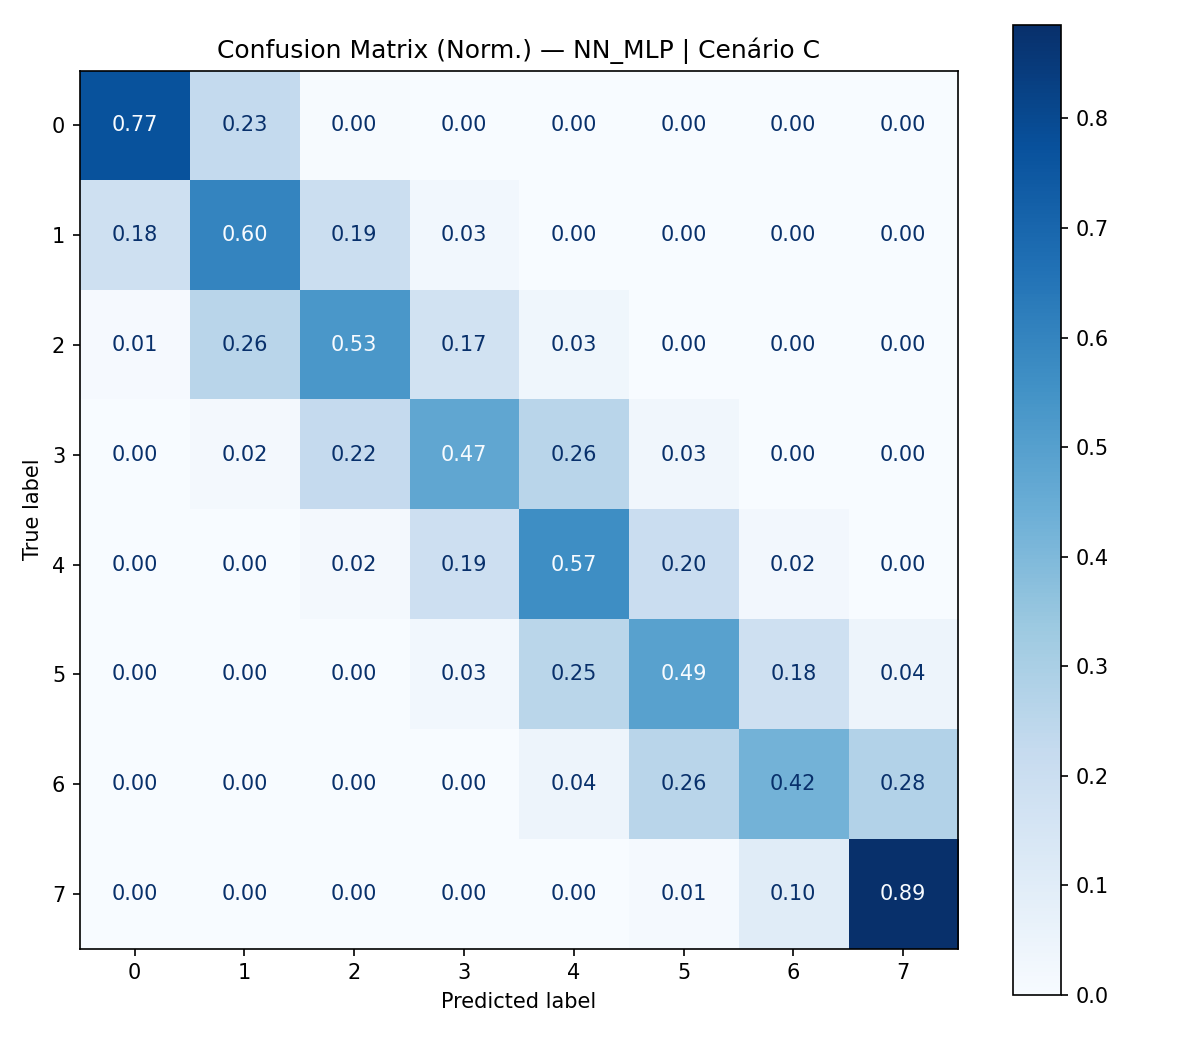
\includegraphics[width=\textwidth]{../graficos/cm_nn_mlp_C.png}
  \caption{NN/MLP}
\end{subfigure}
\begin{subfigure}{0.32\textwidth}
  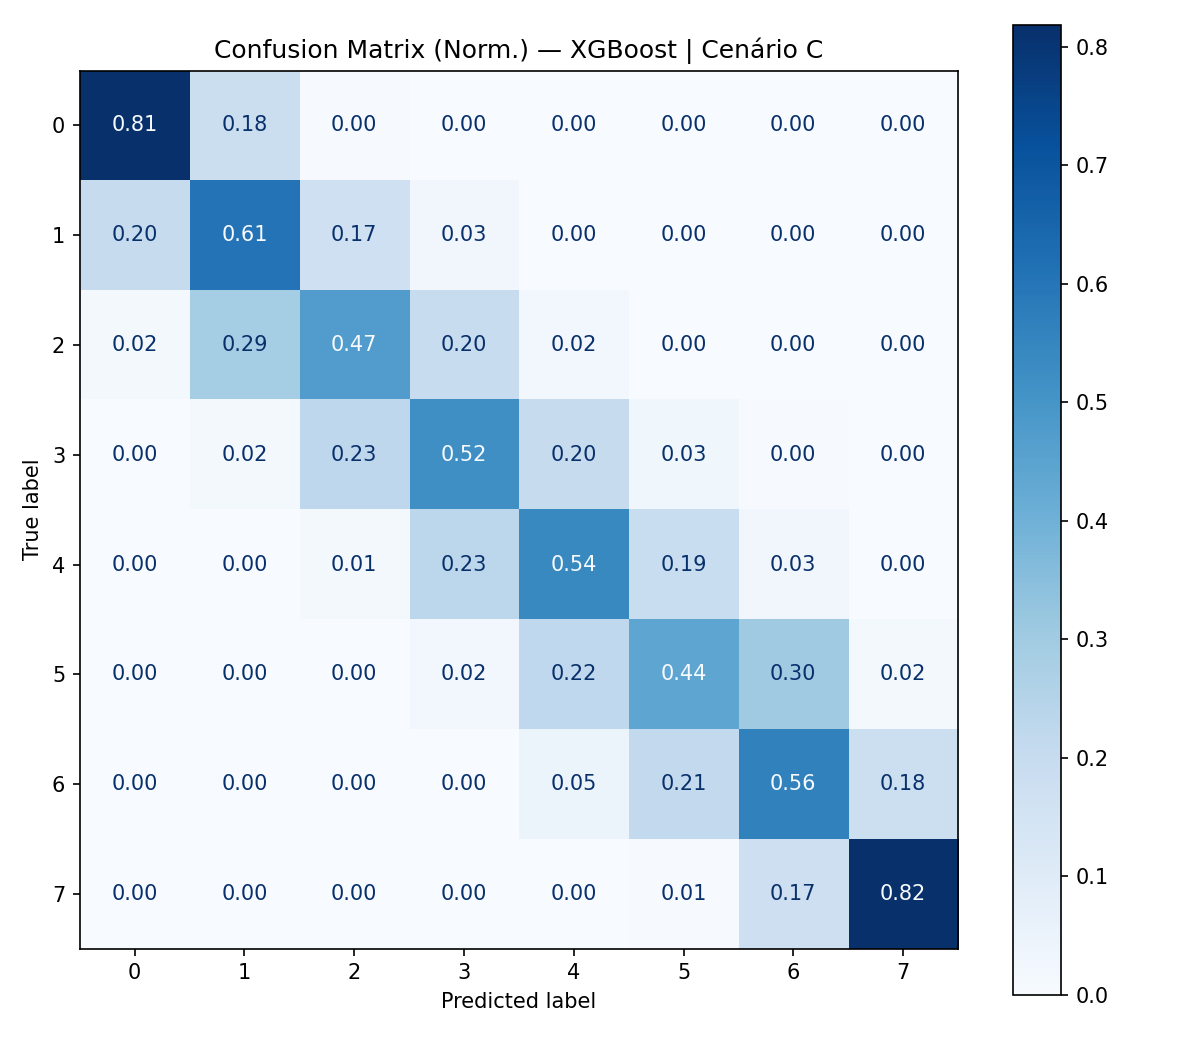
\includegraphics[width=\textwidth]{../graficos/cm_xgboost_C.png}
  \caption{XGBoost}
\end{subfigure}
\caption{Confusion matrices normalizadas -- Cenário C (10 Classes).}
\end{figure}

\subsection{Curvas de Loss -- Rede Neuronal}

\begin{figure}[H]
\centering
\begin{subfigure}{0.32\textwidth}
  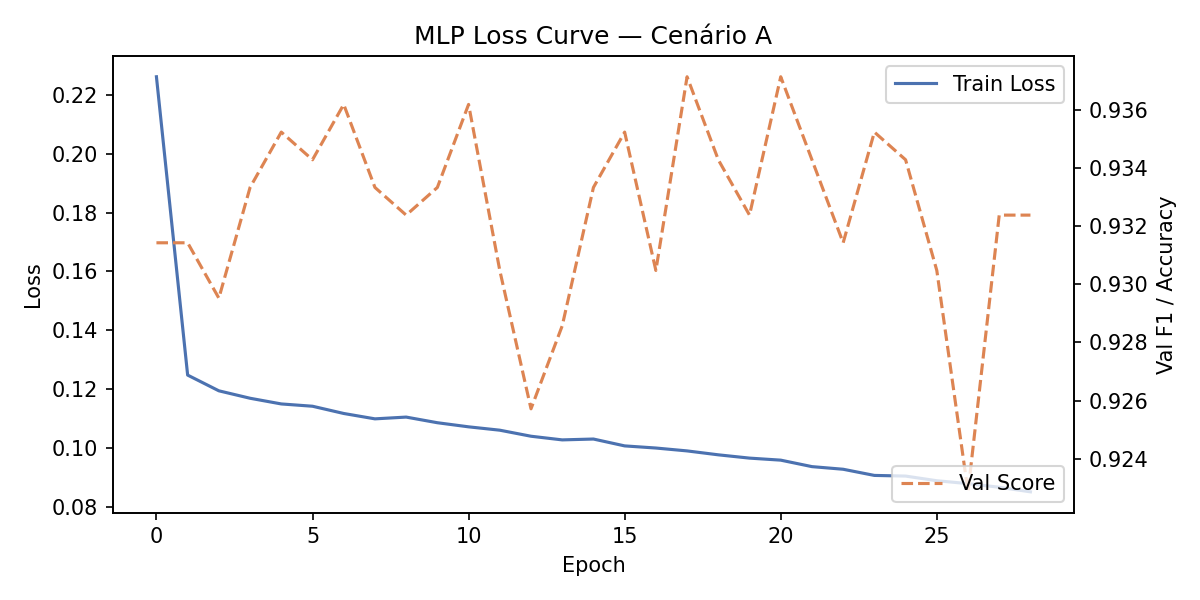
\includegraphics[width=\textwidth]{../graficos/loss_curve_nn_A.png}
  \caption{Cenário A}
\end{subfigure}
\begin{subfigure}{0.32\textwidth}
  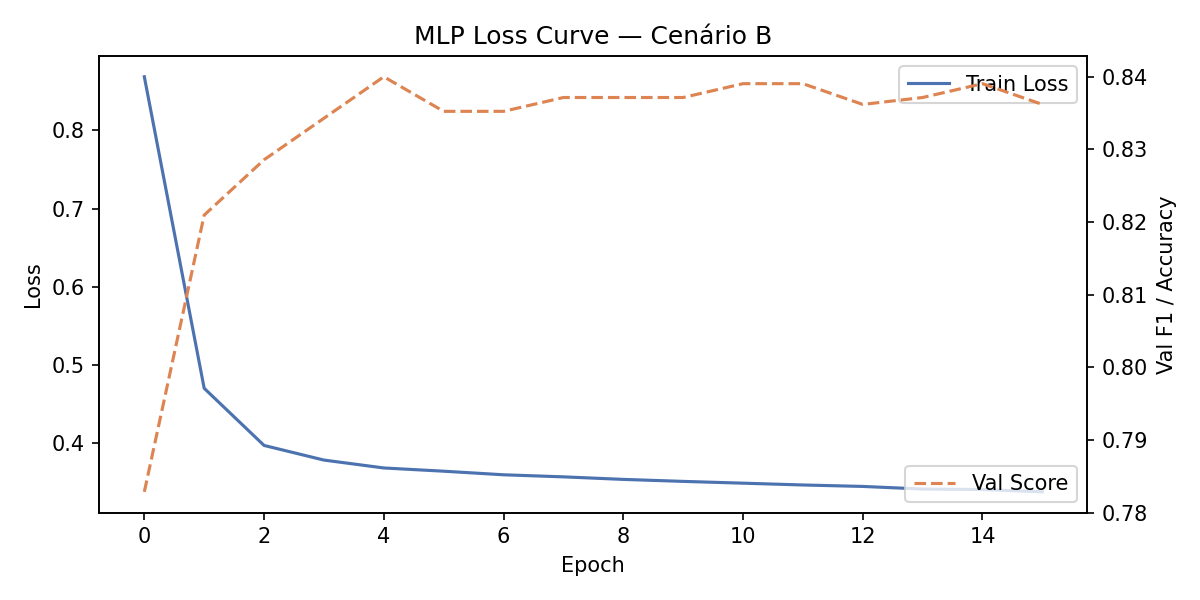
\includegraphics[width=\textwidth]{../graficos/loss_curve_nn_B.png}
  \caption{Cenário B}
\end{subfigure}
\begin{subfigure}{0.32\textwidth}
  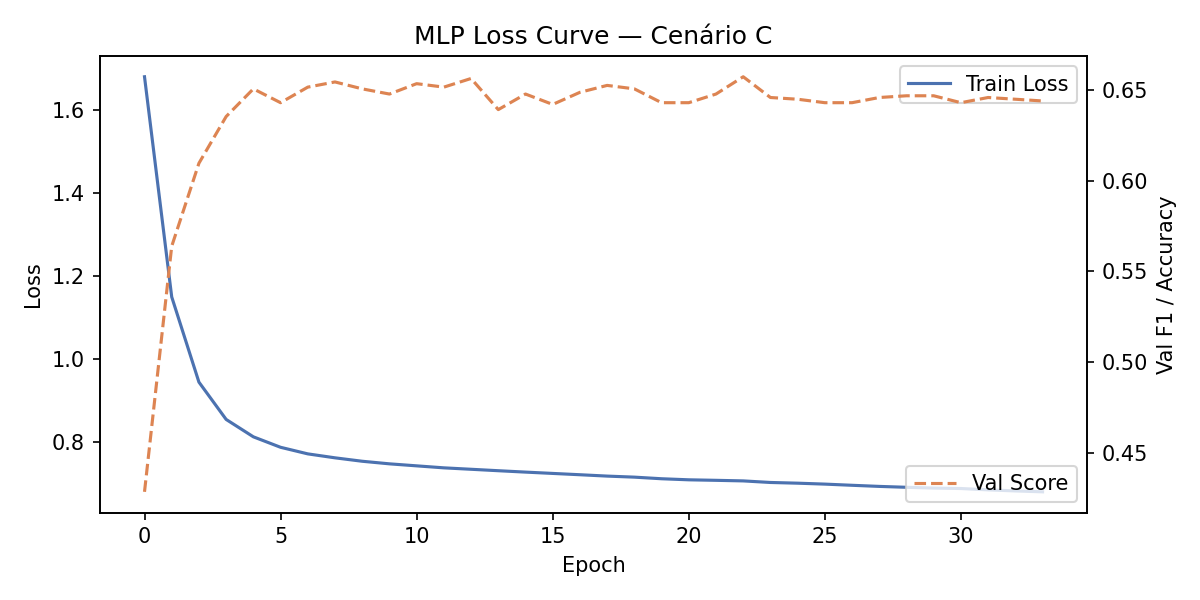
\includegraphics[width=\textwidth]{../graficos/loss_curve_nn_C.png}
  \caption{Cenário C}
\end{subfigure}
\caption{Curvas de loss da MLP nos três cenários. A convergência rápida e a ausência de divergência indicam treino estável.}
\end{figure}

%=============================================================
\section{Análise Crítica dos Resultados}
%=============================================================

\subsection{Cenário A -- Classificação Binária}

Os três modelos atingem F1 macro entre 0.939 e 0.946, o que representa um
\textbf{desempenho excelente}. O problema binário é relativamente simples
dado que o dataset foi construído com uma fronteira de decisão clara.

O \textbf{XGBoost} supera ligeiramente os outros modelos (F1=0.946), sugerindo
que as interações não-lineares entre features são melhor capturadas por árvores
do que por um hiperplano (SVM linear ótimo) ou rede neuronal pequena.

A confusion matrix do Cenário A revela erros simétricos entre as duas classes
($\approx$5\% FP e $\approx$4\% FN), o que confirma que o modelo não está
enviesado para nenhuma classe -- resultado direto do \texttt{class\_weight='balanced'}.

\subsection{Cenário B -- 5 Classes}

O desempenho cai para F1 $\approx$ 0.80--0.81, o esperado num problema multiclasse
com 5 classes. A análise das confusion matrices revela:
\begin{itemize}
  \item \textbf{Classes 0 e 3} (extremos) são classificadas com maior precisão
    ($\approx$87--95\%), pois têm características mais distintas;
  \item \textbf{Classes 1 e 2} (intermédias) são confundidas entre si (F1$\approx$0.72--0.73),
    o que é estruturalmente esperado: instâncias de stress ``baixo'' e ``moderado''
    têm padrões muito semelhantes no espaço de features.
\end{itemize}

O \textbf{SVM tuned} obtém o melhor F1 (0.812), provavelmente porque o kernel linear
(escolhido pelo GridSearch) produz fronteiras de decisão mais robustas para estas
classes adjacentes do que o XGBoost, que tende a sobre-ajustar em regiões de fronteira.

\subsection{Cenário C -- Trade-offs de Granularidade (10 Classes)}

No Cenário C, ao lidar com 10 classes de Stress, o \textit{F1 macro} descende perigosamente de $\approx$0.81 (Cenário B) para apenas $\approx$0.59 nos três modelos. Tal queda global não ilustra um defeito da componente de treino, mas manifesta o \textbf{trade-off inerente entre a complexidade de granularidade e a precisão do diagnóstico}. 

Esta descida de eficácia suportada pelas métricas de classificação é esperada teoricamente e acontece porque:
\begin{enumerate}
  \item \textbf{Sobreposição Espacial de Instâncias}: Indivíduos com \textit{Stress de Nível 5} e \textit{Stress de Nível 6} operam de forma interligada na escala comportamental que as variáveis (sono e utilização) expressam. Forçar as ferramentas paramétricas a distinguir diferenças tão minúsculas acentua um fenómeno de instabilidade sistémica em que o modelo tem de \textit{memorizar ruído microscópico} para diferenciar e aprender os contornos exatos (overfitting na fronteira vizinha).
  \item \textbf{Penalização de Erro Severa e Fronteiras Artificiais}: A discretização equitativa (\textit{equal-frequency binning}) fracionou o universo numa grelha estatisticamente coerente que gerou limites artificiais perfeitamente rectilíneos e desprovidos de semântica, forçando a classificação onde nem um humano saberia a resposta correta.
\end{enumerate}

O efeito da complexidade do problema de otimização contínua pode ser corroborado empiricamente visualizando as \textbf{Learning Curves} apresentadas na Figura \ref{fig:learning_curves_tradeoff}. Ao acompanharmos os eixos verticais consoante progredimos do Cenário A ao Cenário C, comprova-se numéricamente que o limite assintótico e limite máximo global desce invariavelmente (de $\sim 0.94$ para $\sim 0.60$), independentemente do volume de base de dados recolhida. A ausência de discrepância exagerada entre \textit{Training Score} e \textit{Validation Score} nos três gráficos assegura que não existe \textit{overfitting} grosseiro mas uma mera incapacidade base do \textit{espaço de Bayes} perante a tarefa. A eficácia real pode ser confirmada verificando que, se considerássemos os resultados \textit{Top-2 Accuracy}, a acuidade subiria novamente aos abundantes $>$85\%.

\begin{figure}[H]
  \centering
  \begin{subfigure}{0.32\textwidth}
    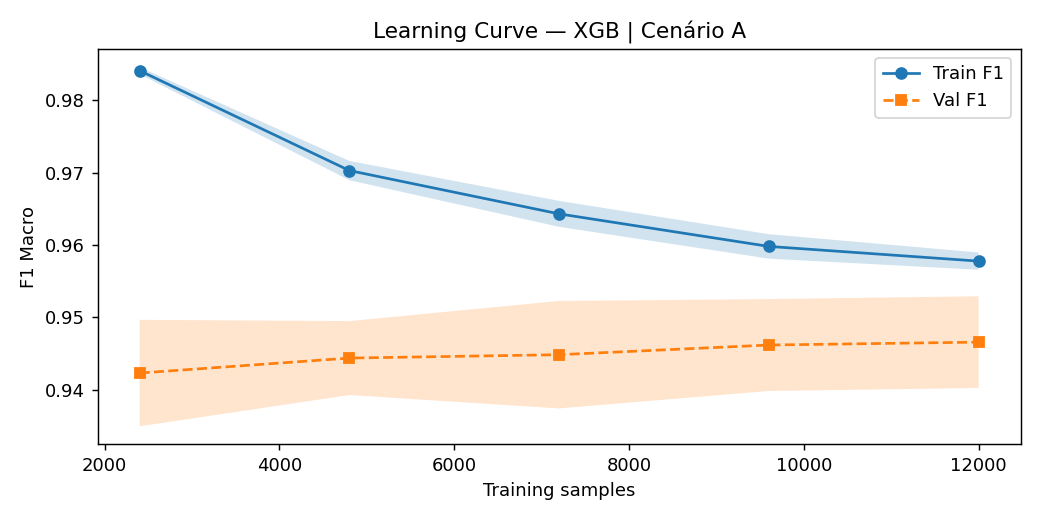
\includegraphics[width=\textwidth]{../graficos/learning_curve_xgb_A.png}
    \caption{Cenário A}
  \end{subfigure}
  \begin{subfigure}{0.32\textwidth}
    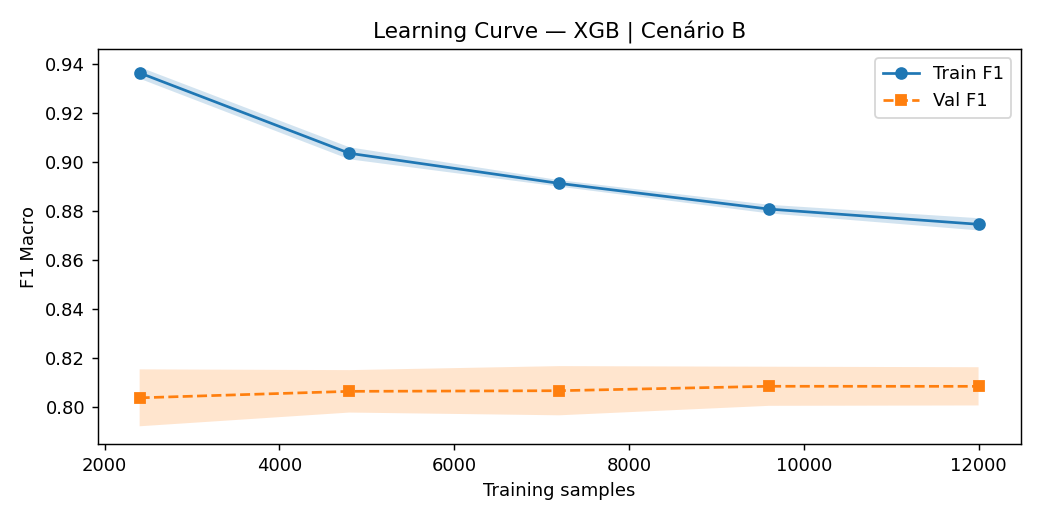
\includegraphics[width=\textwidth]{../graficos/learning_curve_xgb_B.png}
    \caption{Cenário B}
  \end{subfigure}
  \begin{subfigure}{0.32\textwidth}
    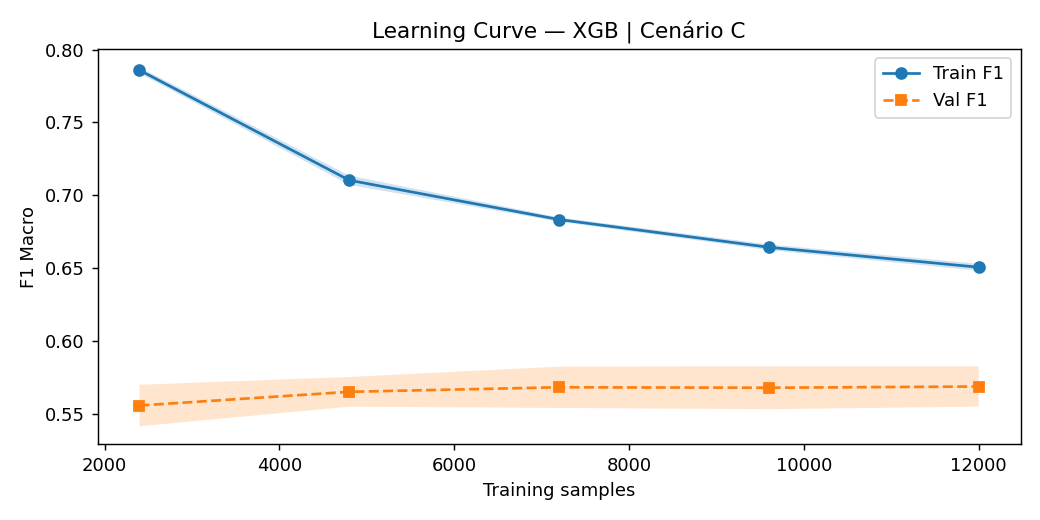
\includegraphics[width=\textwidth]{../graficos/learning_curve_xgb_C.png}
    \caption{Cenário C}
  \end{subfigure}
  \caption{Learning Curves do XGBoost. O gráfico corrobora quantitativamente o trade-off prático do problema de classificação de 10 classes: o patamar máximo de estabilidade (Score médio $\sim 0.60$) é incontestavelmente menor comparativamente aos cenários mais modestos da esquerda.}
  \label{fig:learning_curves_tradeoff}
\end{figure}

\subsection{Comparação entre Modelos}

\begin{itemize}
  \item \textbf{SVM}: consistentemente competitivo, especialmente no Cenário B.
    O kernel linear escolhido pelo GridSearch sugere que o espaço de features
    (após normalização) é aproximadamente linearmente separável. Computacionalmente
    mais pesado -- o SVC com kernel RBF escala como $O(n^2)$ no treino.
  \item \textbf{NN/MLP}: desempenho ligeiramente inferior aos outros dois modelos.
    Com apenas duas camadas ocultas e sem Dropout real (apenas L2), a capacidade
    de generalização é limitada. Uma arquitectura PyTorch com Dropout e mais épocas
    provavelmente melhoraria os resultados.
  \item \textbf{XGBoost}: melhor ou igual ao SVM no Cenário A e C; ligeiramente
    inferior no Cenário B. A invariância à escala e o early stopping tornam-no
    o modelo mais robusto e eficiente a treinar.
\end{itemize}

\subsection{Efeito do Tuning}

A melhoria do tuning face ao baseline é modesta ($+$0.5--1.5\% F1), o que indica
que os hiperparâmetros default são razoáveis para este dataset. A principal
contribuição do GridSearch/RandomizedSearch é a seleção do kernel linear no SVM
(face ao RBF default), que se revelou mais adequado para os Cenários B e C.

\subsection{Interpretabilidade Local (SHAP)}

A necessidade de fundamentar diagnósticos e previsões nas ciências comportamentais médicas prescreve o imperativo de desenvolver métodos matemáticos transparentes. Para colmatar o caráter denso do conjunto e justificar cada decisão, executou-se a auditoria com a métrica \textbf{SHAP (SHapley Additive exPlanations)} com resultados gráficos visíveis (Figura \ref{fig:shap_xgb}). Como indicado numericamente nas posições à direita do eixo central e na intensidade em tons vermelhos, a métrica SHAP verifica positivamente o pressuposto que altos fatores de \texttt{mental\_fatigue\_score} empurram implacavelmente o indivíduo num percurso matemático direcionado a um \textit{output} de Stress superior.

\begin{figure}[H]
  \centering
  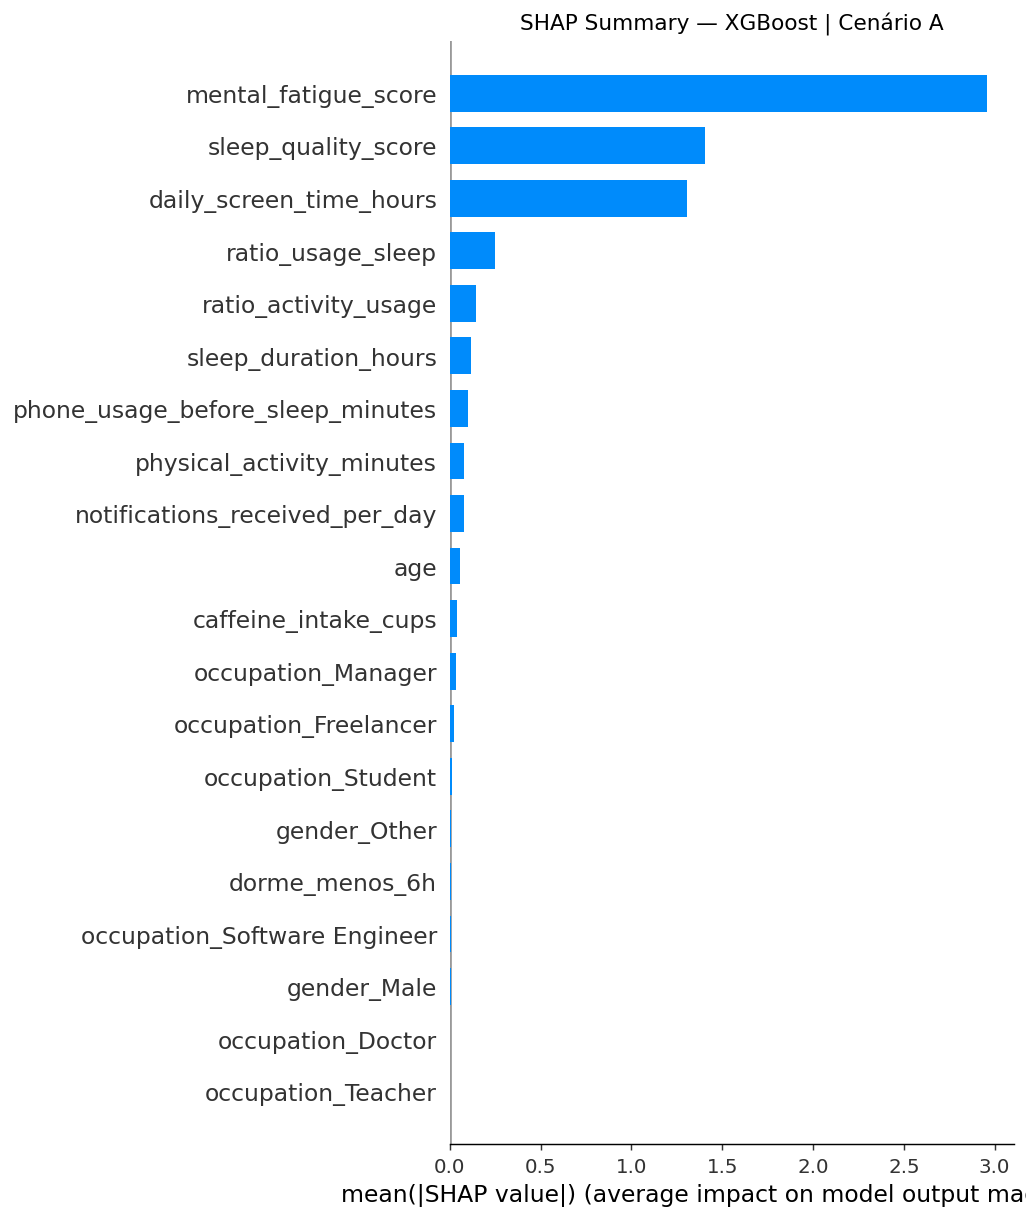
\includegraphics[width=0.7\textwidth]{../graficos/shap_xgb_A.png}
  \caption{Gráfico SHAP Summary para XGBoost (Cenário A). Suporta materialmente com dados locais a evidência estatística em massa do projeto e dita o sentido lógico direto que a fadiga mental opera no stress e target avaliado.}
  \label{fig:shap_xgb}
\end{figure}

\subsection{Limitações e o Desafio do Mundo Real}

O aspeto mais fulcral e que dita uma atitude crítica nas conclusões extraídas deste protótipo, está ligado inteiramente ao meio de origem dos vetores que formam a nossa amostra (\textbf{dados sintéticos}). Os dados sintéticos são fabricados de acordo com diretrizes de ruído estatístico gaussianas ou perfeitamente modeladas que facilitam radicalmente os contornos do padrão alvo do classificador, viabilizando resultados quase-milagrosos na ordem dos $\approx$ 94\% para classes binárias.

A implantação desta arquitetura preditiva em circuitos informáticos ligados a sensores diários num \textbf{mundo real e imprevisível} sofreria colisões extremas contra fatores não modelados:
\begin{itemize}
  \item \textbf{Aparecimento Súbito de Ruído e Erros (Missing Values)}: Num ambiente \textit{in the wild}, os sensores biométricos de um \textit{smartwatch} falham medições por bateria ou posição originando vastos espaços de colunas nulas. Os modelos presentes, instruídos num clima puritano que desconhece ruídos, estatelar-se-iam sob a imprevisibilidade contínua do uso de um sujeito instável.
  \item \textbf{Subjetividade Clínica Severa}: A variável dependente deste dataset é derivada duma perceção pessoal. Pessoas distintas reagem e medem o cansaço moral e o stress sentindo e classificando sintomas com disparidade dramática, criando ambiguidades semânticas que resultam num \textit{Bayes Error} elevadíssimo. Não seria possível reter estatisticamente os F1-Scores de testagem atingidos por causa desta falha epistemológica humana incontornável da variável-alvo na realidade.
  \item O \textbf{Regime de Classes do Cenário C} não passará dum protótipo falhado, devendo re-estruturar-se a grelha de avaliações em 10 níveis estritos para um problema fluido com algoritmos baseados em regressões de quantis (\textbf{Regressão Ordinal}).
\end{itemize}

%=============================================================
\section{Conclusões}
%=============================================================

Este projeto demonstrou a aplicação sistemática de três paradigmas de ML
a um problema de classificação de stress em três cenários de complexidade crescente.

Os principais resultados são:
\begin{itemize}
  \item F1 macro de $\approx$0.94 no Cenário A -- classificação binária robusta;
  \item F1 macro de $\approx$0.80 no Cenário B -- multiclasse com confusão esperada
    nas classes intermédias;
  \item F1 macro de $\approx$0.59 no Cenário C -- limitado pela granularidade de
    10 classes num espaço contínuo.
\end{itemize}

O \textbf{XGBoost} revelou-se o modelo mais equilibrado em desempenho e eficiência.
O \textbf{SVM} destaca-se no Cenário B. A \textbf{NN/MLP} apresenta o desempenho
mais baixo mas oferece maior flexibilidade para arquitecturas mais profundas.

%=============================================================
\section*{Acknowledgements / AI Disclaimer}
%=============================================================

O assistente de IA \textbf{Antigravity (Google DeepMind)} foi utilizado para
auxiliar na geração de código Python (scripts \texttt{main.py}, \texttt{phase2.py},
\texttt{model\_svm.py}, \texttt{model\_nn.py}, \texttt{model\_xgboost.py},
\texttt{utils.py}) e na produção de um rascunho deste relatório LaTeX.
Toda a análise crítica, decisões metodológicas e interpretação dos resultados
foram revistas e validadas pelo autor.

%=============================================================
\begin{thebibliography}{9}

\bibitem{cortes1995}
Cortes, C. \& Vapnik, V. (1995).
Support-vector networks.
\textit{Machine Learning}, 20(3), 273--297.

\bibitem{rumelhart1986}
Rumelhart, D., Hinton, G. \& Williams, R. (1986).
Learning representations by back-propagating errors.
\textit{Nature}, 323, 533--536.

\bibitem{chen2016}
Chen, T. \& Guestrin, C. (2016).
XGBoost: A Scalable Tree Boosting System.
\textit{Proceedings of the 22nd ACM SIGKDD}, pp.~785--794.

\bibitem{shwartz2022}
Shwartz-Ziv, R. \& Armon, A. (2022).
Tabular data: Deep learning is not all you need.
\textit{Information Fusion}, 81, 84--90.

\bibitem{pedregosa2011}
Pedregosa, F. et al. (2011).
Scikit-learn: Machine Learning in Python.
\textit{JMLR}, 12, 2825--2830.

\bibitem{kaggle}
JayJoshi37 (2024).
Sleep, Screen Time and Stress Analysis.
Kaggle. \url{https://www.kaggle.com/datasets/jayjoshi37/sleep-screen-time-and-stress-analysis}

\end{thebibliography}

\end{document}
